% !TEX TS-program = xepythontex



\documentclass[10pt,envcountsect,spanish]{beamer}


\newif\ifnotas
\notasfalse% Para no mostrar los globos
\notastrue % Para  mostrar los globos

\input ../preambulo.tex



%································ TITULO, AUTOR, ETC
\title{Abstracción. Tipos de Datos Abstractos}
\subtitle{Tecnología de la Programación}


\author[L. Daniel Hernández]{L. Daniel Hernández $<ldaniel@um.es>$}

\institute[ldaniel@um.es]{Dpto. Ingeniería de la Información  y las Comunicaciones\\ Universidad de Murcia\\\today\\\,\\\hrule} %	 \\ \today\\ \hrule}


\date[ldaniel@um.es]{ 
\vskip 1.25cm
%\vskip -1.25cm
%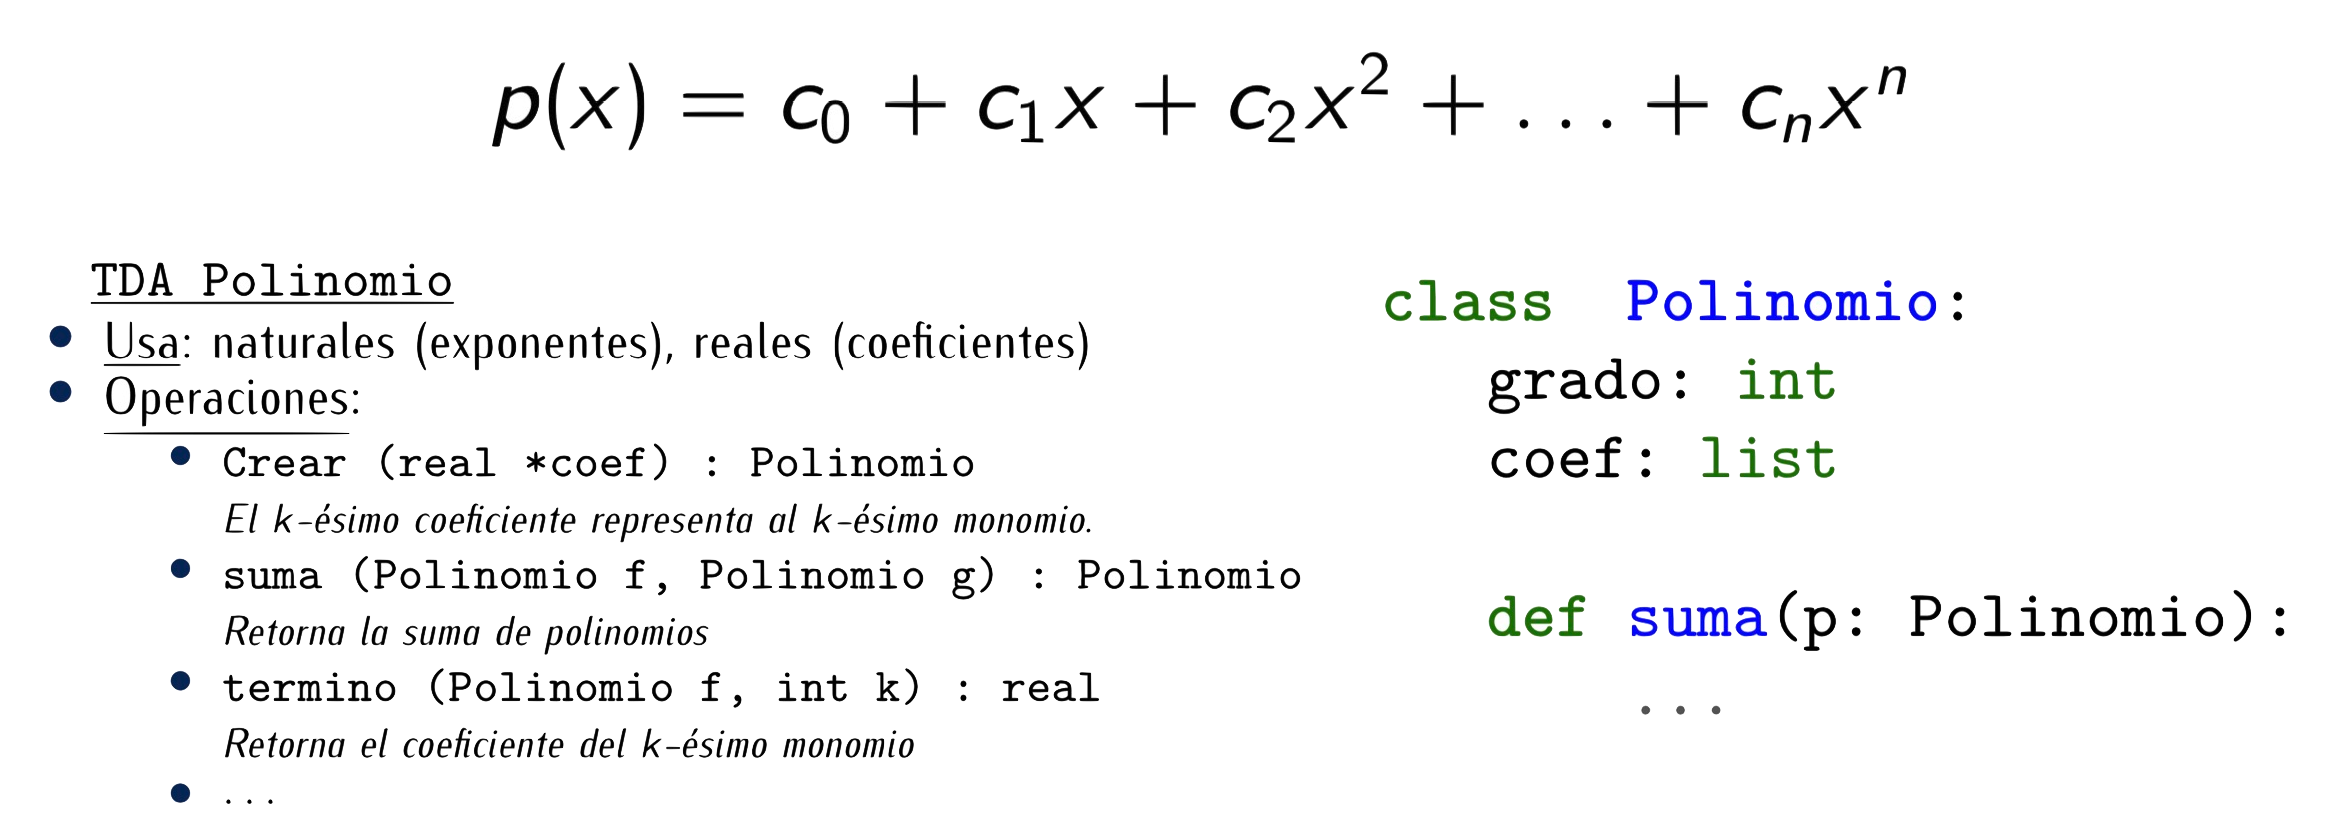
\includegraphics[width=.8\textwidth, height=.18\textheight]{fig/polinomio}
}

\graphicspath{{img/}}



%%%%%%%%%%%%%%%%%%%%%%%%%%%%%%%%%%
%%%%%%%%%%%%%%%%%%%%%%%%%%%%%%%%%%
%%%%%%%%%%%%%%%%%%%%%%%%%%%%%%%%%%
%%%%%%%%%%%%%%%%%%%%%%%%%%%%%%%%%%

%https://es.overleaf.com/learn/how-to/Writing_Markdown_in_LaTeX_Documents
\usepackage[hashEnumerators]{markdown}


%%%%%%%%%%%%%%%%%%%%%%%%%%%%%%%%%%
%%%%%%%%%%%%%%%%%%%%%%%%%%%%%%%%%%
%%%%%%%%%%%%%%%%%%%%%%%%%%%%%%%%%%
%%%%%%%%%%%%%%%%%%%%%%%%%%%%%%%%%%
\begin{document}

%\pgfdeclareimage[height=1cm]{logo}{logo.png}
%\logo{\pgfuseimage{logo}}



%--------------------------------------------------------------------------------
{\usebackgroundtemplate{%
  \includegraphics[width=\paperwidth,height=\paperheight]{../img/fondoUMUCompleto}}
\begin{frame}[b]
	\maketitle

\begin{tikzpicture}[overlay, remember picture]
\node[anchor=south west, %anchor is bottom left corner of the graphic
      xshift=.2\textwidth, %shifting around
      yshift=0.7cm] 
     at (current page.south west) %left bottom corner of the page
     {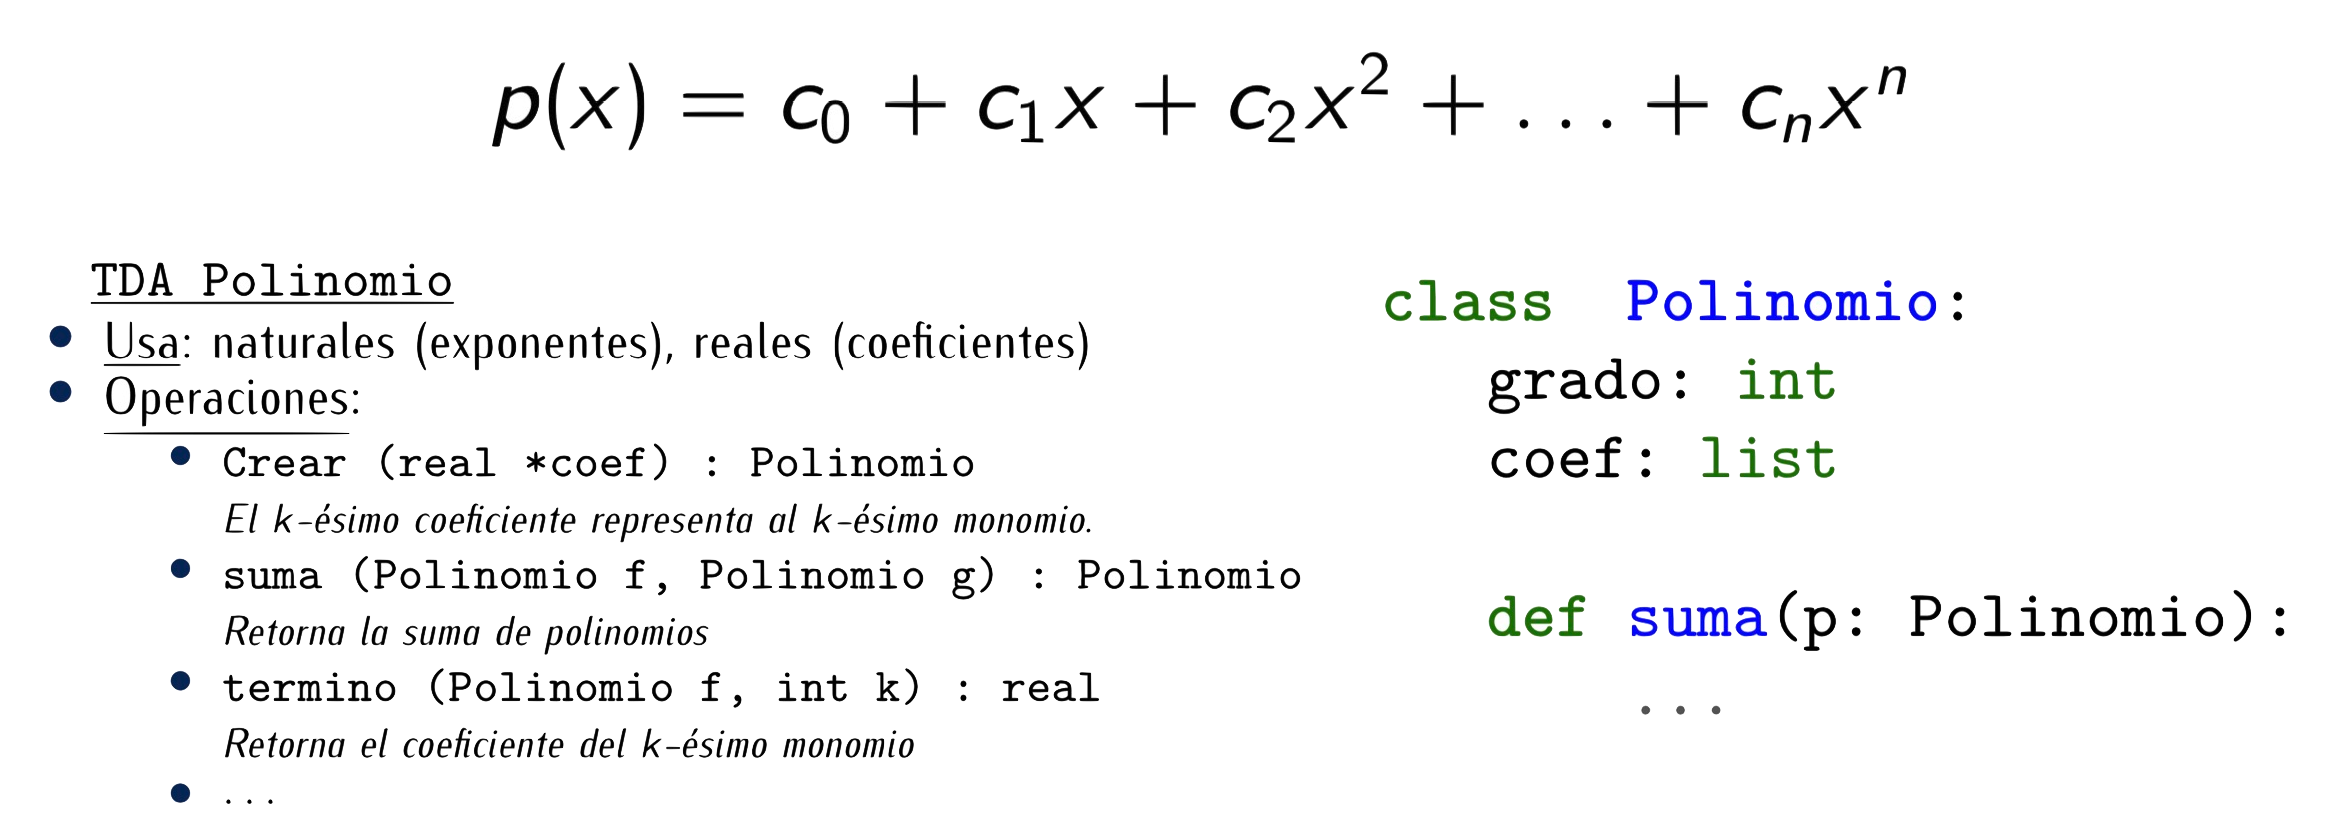
\includegraphics[width=.8\textwidth, height=.3\textheight]{fig/polinomio}}; 
\end{tikzpicture}
	
\end{frame}			% Transparencia: Título
}



%--------------------------------------------------------------------------------
%%%%%%%%%%%%%%%%%%%%%%%%%%%%%%%%%%
%%%%%%%%%%%%%%%%%%%%%%%%%%%%%%%%%%
\begin{frame}{Índice de Contenidos}\tableofcontents \end{frame}


%%%%%%%%%%%%%%%%%%%%%%%%%%%%%%%%%%%%%
%%%%%%%%%%%%%%%  SECTION   %%%%%%%%%%%%%%%
%%%%%%%%%%%%%%%%%%%%%%%%%%%%%%%%%%%%%
\section{Abstracción}


%%%%%%%%%%%%%%%%%%%%%%%%%%%%%%%%%%
%%%%%%%%%%%%%%%%%%%%%%%%%%%%%%%%%%
\begin{frame}{Abstracción}

\begin{itemize}%\setlength{\itemsep}{0mm}

\item 
La \key{abstracción}  es el proceso mental por el que captamos las \key[red]{características principales} de un concepto o proceso descartando los detalles aíslando conceptualmente las distintas partes, propiedades o cualidades de un objeto para estudiarlas por separado. 

\item 
Este proceso categoriza elementos en grupos.  

\begin{itemize}
	\item 
	Cada grupo es una abstracción que ignora determinadas características de los elementos que forman parte del grupo

	\item 
	Pero a la vez, en cada grupo, se resalta los aspectos más relevantes de los objetos que contienen.
\end{itemize}


\item La abstracción permite estudiar un sistema complejo a diferentes niveles de detalle; es decir, refleja un \key{modelo jerárquico}. 

La abstracción permite hacer una descomposición en la que varía el nivel de detalle.
\textit{Ej: Desde el concepto de bisagra al concepto de vivienda.}


\item 
Es muy importante que cada uno de los niveles de abstracción estén al mismo nivel. 
\end{itemize}

\end{frame}




%%%%%%%%%%%%%%%%%%%%%%%%%%%%%%%%%%%%%
%%%%%%%%%%%%%%%  SECTION   %%%%%%%%%%%%%%%
%%%%%%%%%%%%%%%%%%%%%%%%%%%%%%%%%%%%%
\section{Mecanismos de Abstracción}

%%%%%%%%%%%%%%%%%%%%%%%%%%%%%%%%%%
%%%%%%%%%%%%%%%%%%%%%%%%%%%%%%%%%%
\begin{frame}[fragile]{Mecanismos de Abstracción}{Métodos prácticos que se emplean}

\begin{itemize}
\item \key{Abstracción por parametrización.}

\begin{itemize}

\item 
Un parámetro representa a un conjunto de elementos específicos. 

\unEjemplo \pyv{int num}, que es una abtracción de los valores concretos naturales 1, 2, 3, ... con los que podemos identificar \pyv{num}.

\item 
Los parámetros se usan en los procedimientos (abstracción procedimental): los parámetros en un función/procedimiento, abstrae un número infinito de acciones.

\unEjemplo: En vez de usar el procedimiento \cm{trasladarAlPunto(\cm{juan, (1, 3)})} se puede usar  \cm{trasladarAlPunto(\cm{Objeto obj, Punto p})} para representar que se quiere trasladar cualquier objeto a un punto del plano (y no solo a \texttt{juan} a un punto concreto).  

\end{itemize}




\item \key{Abstracción por especificación.} Se basa en cumplimentar un documento en el que se indica lo siguiente:
\begin{itemize}
\item Un nombre. El identificador de un procedimiento, función, ...

\item Una descripción.~Explica en qué consiste la  abstracción pero  solo mencionará lo imprescindible. 

\item Las condiciones. Los estados que deben cumplirse. Varias partes según los detalles de la abstracción a realizar. 

\unEjemplo En una abstracción procedimental, se debe determinar, al menos,  las \textbf{precondiciones} (los requisito exigidos para el procedimiento) y las \textbf{postcondiciones} (el efecto de la ejecución).

\end{itemize}

\end{itemize}

\end{frame}




%%%%%%%%%%%%%%%%%%%%%%%%%%%%%%%%%%%%%
%%%%%%%%%%%%%%%  SECTION   %%%%%%%%%%%%%%%
%%%%%%%%%%%%%%%%%%%%%%%%%%%%%%%%%%%%%
\section{Tipos de Abstracción}

%%%%%%%%%%%%%%%%%%%%%%%%%%%%%%%%%%
%%%%%%%%%%%%%%%%%%%%%%%%%%%%%%%%%%
\begin{frame}[fragile]{Tipos de Abstracción}


\begin{itemize}%\setlength{\itemsep}{0mm} \footnotesize
\item \key{Abstracción procedimental.} Es definir un conjunto de\textbf{ procedimientos como abstracción de operaciones}. 

\begin{itemize}
\item 
Funciones y procedimientos responden a esta abstracción.

\item 
\textit{\footnotesize Ej: la suma de números se abstrae para sumar matrices, listas, ...}
\end{itemize}


\item \key{Abstracción de iteración.} Es la que usa \textbf{colecciones} de objetos \textbf{y} permite \textbf{pasar de un elemento al siguiente} sin saber cómo se organizan de forma interna. 

\begin{itemize}
\item 
Intervienen dos elementos: el \textbf{iterable} y el \textbf{iterador}.

\item \textit{\footnotesize Ej: \cm{while(vector.hasNext())} generaliza  a \cm{while( i < len(vector) )}, pues ya no depende del índice y solo depende de la colección.}
\end{itemize}


\item \key{Abstracción de datos.} Es la que trabaja con \textbf{conjunto de objetos y  conjunto de operaciones} (procedimientos) sobre los objetos, lo que los dota de un comportamiento. 

\begin{itemize}
\item La mayor abstracción define modelos: datos + operaciones

\item 
\textit{Ej: la estructura de grupo en matemáticas es una abstracción de cualquier conjunto de objetos que tenga un operador cerrado con ciertas propiedades.  No importa cuáles son los objetos de la estructura.}
\end{itemize}


\end{itemize}

\end{frame}



%%%%%%%%%%%%%%%%%%%%%%%%%%%%%%%%%%
%%%%%%%%%%%%%%%%%%%%%%%%%%%%%%%%%%
\subsection{Abstracción Procedimental}

%%%%%%%%%%%%%%%%%%%%%%%%%%%%%%%%%%
%%%%%%%%%%%%%%%%%%%%%%%%%%%%%%%%%%
\begin{frame}[fragile]{Abstracción Procedimental}
%\small 
\begin{itemize}% \setlength{\itemsep}{0mm}
\item Consiste en crear \key{procedimientos y funciones} como abstracción de operaciones.

\item Un procedimiento/función \textbf{debe responder sin ambigüedad a \key{qué} hace obviando el \key{cómo} lo implementa.}

\item Abstraemos un conjunto de operaciones (detalles de cómo se realiza) como una única operación (el qué hace), expresada como función o procedimiento.

\item Las técnicas de \key{programación procedimental y modular} usan este tipo de abstracción para romper el problema principal en problemas más pequeños.
\item Toda operación  \key{se debe especificar} de la siguiente forma:
\small
\begin{Verbatim}[frame=single]
operacion nombre (id1:tipo1, id2: tipo2, ....) return tipo
    Precondiciones: Indican los datos de entrada, los id
    Retorna: Indica el tipo de dato que retorna
    Descripción: Descripción textual del comportamiento de 
                 la operación (el efecto)
    Excepciones: Indica las excepciones (opcional)
\end{Verbatim}

\item Este tipo de especificaciones los incorporan los IDE y editores de programación.

\item A partir de estas especificaciones se genera la documentación (API) para los programadores.
Un buen ejemplo es  
%\textcolor{blue}{\huge \ComputerMouse}  
\url{https://docs.oracle.com/javase/7/docs/api/java/lang/String.html#substring(int)}
\end{itemize}
\end{frame}


%%%%%%%%%%%%%%%%%%%%%%%%%%%%%%%%%%
%%%%%%%%%%%%%%%%%%%%%%%%%%%%%%%%%%
\subsection{Abstracción de Iteración}
%%%%%%%%%%%%%%%%%%%%%%%%%%%%%%%%%%
%%%%%%%%%%%%%%%%%%%%%%%%%%%%%%%%%%
\begin{frame}[fragile]{Abstracción de Iteración}
%\small 
\begin{itemize}% \setlength{\itemsep}{0mm}
\item Consiste en tener algún mecanismo que permita \key{acceder} a los elementos de un contenedor \key{sin tener en cuenta su representación interna}.

\item \textbf{Representación interna}: Estructura de datos que se utiliza para representar al contenedor.

\item Los \key{bucles con contadores} tienen en cuenta la representación de los datos.
\begin{Verbatim}[frame=single, fontsize=\footnotesize]
for i: int = 0...top:
    acción sobre elemento[i] # Considera estructura indexada
\end{Verbatim}

\item Es más adecuado tener una \key{abstracción} de la forma:

\begin{Verbatim}[frame=single, fontsize=\footnotesize]
for cada elemento P de Contenedor
    acción sobre P
\end{Verbatim}

\item La responsabilidad del recorrido se traslada a un objeto que se llamará \key{iterador}.

\item Sobre un contenedor se podría definir \key{diferentes iteradores}:

\begin{itemize}
\item
Cada iterador sabe cómo recorrer el contenedor para el que se define 

\item
Cada iterador tiene su propio recorrido sobre la estructura
\end{itemize}

\item Sobre distintos tipos de contenedores los iteradores puede recorrerlas usando una \key{interfaz común}:\textbf{ !`no hay que cambiar el código principal! }P.e. \cm{iterador.next()}
\end{itemize}
\end{frame}



%%%%%%%%%%%%%%%%%%%%%%%%%%%%%%%%%%
%%%%%%%%%%%%%%%%%%%%%%%%%%%%%%%%%%
\subsection{Abstracción de Datos}
%%%%%%%%%%%%%%%%%%%%%%%%%%%%%%%%%%
%%%%%%%%%%%%%%%%%%%%%%%%%%%%%%%%%%
\begin{frame}{Abstracción de Datos}
\begin{itemize}% \setlength{\itemsep}{0mm}
\item Existen 3 tipos (o niveles) de abstracción.
\item \key{Tipos de datos integrados}  (o fundamentales). Son los que ofrecen los lenguajes de programación.

\cm[magenta]{Ejemplo:} En \cm[red]{Python} se distinguen, entre otros\footnote[frame]{\url{https://docs.python.org/es/3/library/stdtypes.html}}:
\begin{itemize}
\item Los tipos de datos simples: numéricos (enteros, reales y complejos) y booleanos.
\item Los tipos de datos compuestos: cadena de caracteres (str), secuencias (rangos, listas y tuplas), mapas (diccionarios), conjuntos.
\end{itemize}


\item \key{Tipos de datos definidos por el usuario} o programador. Son los que pueden diseñar los programadores agrupando todos de datos fundamentales. 

\begin{itemize}
\item array, record, struct, \cm{class}
\end{itemize}

\item \key{Tipos de datos abstractos (TDA).} Construye modelos (matemáticos) usando agrupación de datos.

\begin{itemize}
\item No es lo mismo una estructura de datos formado por dos valores y operar con ellos que trabajar con vectores numéricos 2D con operaciones matemáticas (donde no importa la estructura).
\end{itemize}

\end{itemize}

\end{frame}




%%%%%%%%%%%%%%%%%%%%%%%%%%%%%%%%%%
%%%%%%%%%%%%%%%%%%%%%%%%%%%%%%%%%%
\section{Tipos de Datos Abstractos}
%%%%%%%%%%%%%%%%%%%%%%%%%%%%%%%%%%
%%%%%%%%%%%%%%%%%%%%%%%%%%%%%%%%%%
\begin{frame}{Tipos de Datos Abstractos}

\begin{itemize}
\item  Los \key{Tipos de Datos Abstractos} (TDA) son \textbf{modelos matemáticos} que constan de

\begin{itemize}
\item un nombre publico para 
\item identificar a un conjunto de datos (valores), junto con
\item un conjunto de operaciones bien definidas sobre los datos (como en una estructura algebraica). 
\end{itemize}

\item Como modelo, le es \key{irrelevante} cómo se almacenan o estructuren los datos y cómo se implementan las operaciones.

\item Para todo TDA hemos de abordar \key{tres tareas}: 

\begin{itemize}
\item \textbf{Especificación:} definición del TDA 
\item \textbf{Representación:} estructura con la que representar el TDA.
\item \textbf{Implementación:} cómo implementar la estructura en un lenguaje de programación.
\end{itemize}

\end{itemize}
\end{frame}




%%%%%%%%%%%%%%%%%%%%%%%%%%%%%%%%%%
%%%%%%%%%%%%%%%%%%%%%%%%%%%%%%%%%%
\subsection{Especificación de TDAs}
%%%%%%%%%%%%%%%%%%%%%%%%%%%%%%%%%%
%%%%%%%%%%%%%%%%%%%%%%%%%%%%%%%%%%
\begin{frame}{Especificación de TDAs}

\begin{itemize}
\item La \key{especificación} de un TDA (Datos+Operaciones) se rige por las normas generales de la \textit{\bf Abstracción por Especificación}

\item La especificación consta de \key{tres partes}: nombre y descripción, la definición de los datos y la definición de los operadores.

\item \key{Nombre y descripción.}
\begin{itemize}
\item Se le dará un nombre que identifica al conjunto de datos y las operaciones.
\item Se indicará qué representan.
\end{itemize}


\item \key{Especificación de los datos.}
\begin{itemize}

	
\item Pueden venir dados por reglas.

\unEjemplo Definiciones recursivas (p.e. una lista).


\item Puede usar notaciones matemáticas conocidas.

\unEjemplo Conjuntos conocidos ($\mathbb{N}$, $\mathbb{R}$, ...), conjuntos $\{s_1,s_2,\ldots\}$, intervalos $[a, b]$, expresiones regulares, ... 

\item Nunca se definirá pensando en estructuras concretas de un lenguaje de programación. 

\end{itemize}


\item \key{Especificación de las Operaciones} (abstractas).

\begin{itemize}
\item Se indicará tanto la sintaxis como la semántica de cada una. 
\item Se emplearan las especificaciones de la abstracción procedimental.
\end{itemize}


\item \textbf{IMPORTANTE.} \key{Un TDA define un valor de tipo $T$:} 

\centerline{\it Todos los entes/valores que respondan al TDA $T$ son de tipo $T$.}

\end{itemize}
\end{frame}




%%%%%%%%%%%%%%%%%%%%%%%%%%%%%%%%%%
%%%%%%%%%%%%%%%%%%%%%%%%%%%%%%%%%%
\begin{frame}{Tipos de Operadores de los TDAs}
\begin{itemize}% \setlength{\itemsep}{0mm}
\item Los operadores de un TDA se pueden dividir por su \key{objetivo}:

	\begin{itemize}
	\item \key{Constructores.} \\ Los que indican cuáles son los datos necesarios para construir un valor de tipo $T$.
	\item \key{Modificadores.} \\ Los que construyen un nuevo valor de tipo $T$ a partir de un valor de tipo $T$ dado.
	\item \key{Consulta}. \\ El conjunto de operaciones que a partir de un valor de tipo $T$ retornan un valor, que no es de tipo $T$.
	\end{itemize}

\item Las operaciones de un TDA se pueden dividir por su \key{importancia}:

	\begin{itemize}
	\item \key{Fundamentales,} también llamadas primitivas. Cumplen  dos condiciones:

	\begin{itemize}
		\item \textbf{No se puede quitar ninguna:} La supresión de una de ellas conlleva que encontramos problemas que no se pueden resolver porque nos faltan operaciones.
		\item Ese conjunto de operaciones \textbf{permite construir cualquier otro tipo de operación} sobre el TDA.
		\item \textbf{Todas deben poder usarse:} todas deben estar visibles.
	\end{itemize}

	\item \key{No fundamentales.}

	\begin{itemize}
		\item \textbf{Apoyan la definición de una operación fundamental,} pero no se puede considerar como tal. No deben de usarse (deben estar ocultas)
		\item Las que \textbf{aumentan el conjunto de operaciones} y se construyen a partir de fundamentales (deberían añadirse las menos posibles)
	\end{itemize}

	\end{itemize}

\end{itemize}
\end{frame}





%%%%%%%%%%%%%%%%%%%%%%%%%%%%%%%%%%
%%%%%%%%%%%%%%%%%%%%%%%%%%%%%%%%%%
\begin{frame}{Un ejemplo de definición de TDA.}

$ $\hskip-0.5cm   \unEjemplo \texttt{\underline{TDA Polinomio}}
\begin{itemize} \setlength{\itemsep}{0mm}
\item { Es una expresión algebraica {\footnotesize $p(x)=c_0+c_1x+c_2x^2+\ldots+c_nx^n$ } compuesta por la \textbf{suma} de dos o más monomios (es un \textbf{coeficiente} y una \textbf{variable} con \textbf{exponente}).
No existen dos monomios con el mismo exponente. Todos los monomios usan la misma variable. El $k$-ésimo monomio es el que tiene una variable con coeficiente $\not=0$.
}

\item \underline{Usa}: {  naturales (exponentes), reales (coeficientes)}

\item \underline{Operaciones}:
	\begin{itemize} 
	\item \texttt{Crear (real *coef) : Polinomio} \\
		\textit{ El $k$-ésimo coeficiente representa al $k$-ésimo monomio.}

	\item \texttt{suma (Polinomio f, Polinomio g) : Polinomio}\\
		\textit{ Retorna la suma de polinomios}

	\item \texttt{termino (Polinomio f, int k) : real}\\
		\textit{ Retorna el coeficiente del $k$-ésimo monomio}
		
	\item $etc \cdots$
	\end{itemize}


\item \textbf{NOTA.} Aquí se muestra una versión simplificada. Hay que seguir la especificación procedimental.
\end{itemize}



\end{frame}




%%%%%%%%%%%%%%%%%%%%%%%%%%%%%%%%%%
%%%%%%%%%%%%%%%%%%%%%%%%%%%%%%%%%%
%--------------------------------------------------------------------------------
\subsection{Representación de TDAs}


%%%%%%%%%%%%%%%%%%%%%%%%%%%%%%%%%%
%%%%%%%%%%%%%%%%%%%%%%%%%%%%%%%%%%
\begin{frame}[fragile]{Representación de TDAs}

\begin{itemize}
\item Se debe de elegir una estructura \textbf{rep} indicando qué datos de un valor de tipo $T$ se almacenan en la estructura \textbf{rep}.

 
\item \key{La función de abstracción.} Una función sobreyectiva $Abst: \mbox{\textbf{rep}} \longrightarrow {\cal A}$ 

\item \key{El invariante de la representación.} Es un predicado
$I: \mbox{\textbf{rep}} \longrightarrow \mathbb{B}$ que es cierto para los objetos de \textbf{rep} que sean legítimos.


\

\item \unEjemplo \texttt{\underline{Representación de Polinomios}}
\begin{itemize}[nosep]
\item	 Para los polinomios {\small $p(x)=c_0+c_1x+c_2x^2+\ldots+c_nx^n$ }se opta por la estructura:

\hfil \begin{minipage}{.24\textwidth}
\scriptsize \tt
\begin{pyverbatim}[][frame=single]
struct rep {
   entero grado
   real[] coef
}
\end{pyverbatim}
\end{minipage}




\item \texttt{grado} es \key{un entero} para representar el grado del polinomio, y 
\item \texttt{coef} es \key{una lista} indexada de reales para representar a los coeficientes \\
\texttt{coef} NO ES UN ARRAY.
\item {\ttfamily  \footnotesize
$Abst($r$)=$r.coef[0]+r.coef[1]$x$+r.coef[2]$x^2$ + $\ldots$  \\
$ $ \hfill $\ldots$ + r.coef[r.grado]$x^{\mbox{\texttt{r.grado}}} $
}

\item {\ttfamily 
$I($r$)$=(r.grado$\not<$0) AND r.grado = len(r.coef)
}
\end{itemize}
%}

\end{itemize}

\end{frame}






%%%%%%%%%%%%%%%%%%%%%%%%%%%%%%%%%%
%%%%%%%%%%%%%%%%%%%%%%%%%%%%%%%%%%
%--------------------------------------------------------------------------------
\subsection{Implementación de TDAs}

%%%%%%%%%%%%%%%%%%%%%%%%%%%%%%%%%%
%%%%%%%%%%%%%%%%%%%%%%%%%%%%%%%%%%
\begin{frame}{Implementación de TDAs}


\begin{itemize}
\item \underline{\cm{lenguaje}}: lenguaje de programación en el que se  implementa el TDA.
\item Lo que \textbf{necesita conocer} el usuario del TDA en ese \underline{\cm{lenguaje}} es:
	 \small
	\begin{itemize}
	\item su \key{nombre}, 
	\item su \key{dominio} (conjuntos de datos con los que trabaja y su tipo), 
	\item su \key{interface} (los nombres de las operaciones asociadas). 
	\end{itemize}
	
	Estos 3 elementos caracterizan a un TDA y se llama \key[red]{parte pública}.
	\normalsize
	
\item Lo que \textbf{no necesita conocer} el usuario del TDA en ese \underline{\cm{lenguaje}} es:
	\small
	\begin{itemize} 
	\item la \textbf{estructura de datos} usada (cómo está codificados los conjuntos de datos)
	\item cómo se han \textbf{implementado} los algoritmos (operadores)
	\end{itemize}
	
	Estos elementos reciben el nombre de \key[red]{parte privada}.
	\normalsize
	
\item Cuando se programe el TDA se deberá de tener en cuenta estas dos partes.

\item Se deberá de implementar considerando:

	\small
	\begin{itemize} 
	\item \key{Encapsulamiento,} agrupando en un objeto atributos (variables) y métodos (operaciones).
	\item \key{Ocultación} de información, pues establecer qué atributos y métodos pueden permanecer ocultas (o visibles).
	\end{itemize}
	\normalsize
	
	

	
\item La POO aparece de forma natural para resolver esta situación.


\item \small \key[red]{Nuestro Objetivo:} 

\centerline{\bf \underline{Usar} la POO para \underline{implementar} TDAs (que son modelos matemáticos) \underline{en} \cm[red]{Python}.}

\end{itemize}

\end{frame}


\end{document}


